% !TEX program = xelatex
\documentclass[a4paper,14pt,oneside,openany]{memoir}

\usepackage[left=30mm, right=15mm, top=20mm, bottom=20mm]{geometry}
\pagestyle{plain}
\parindent=1.25cm
\usepackage{indentfirst}

\usepackage{polyglossia}
\setdefaultlanguage[indentfirst=true,forceheadingpunctuation=false]{russian}
\setotherlanguages{english}

\IfFontExistsTF{Times New Roman}
{\setmainfont{Times New Roman}
\newfontfamily\cyrillicfont{Times New Roman}[Script=Cyrillic]}
{\setmainfont[Script=Cyrillic]{FreeSerif}}

\IfFontExistsTF{Courier New}
{\setmonofont{Courier New}
\newfontfamily\cyrillicfonttt{Courier New}[Script=Cyrillic]}
{\setmonofont[Script=Cyrillic]{FreeMono}}

\IfFontExistsTF{Arial}
{\setsansfont{Arial}
\newfontfamily\cyrillicfontsf{Arial}[Script=Cyrillic]}
{\setsansfont[Script=Cyrillic]{FreeSans}}

\setsecnumdepth{subsection}
\renewcommand*{\chapterheadstart}{}
\renewcommand*{\printchaptername}{}
\renewcommand*{\chapnumfont}{\normalfont\bfseries}
\renewcommand*{\afterchapternum}{\hspace{1em}}
\renewcommand*{\printchaptertitle}{\normalfont\bfseries\centering\MakeUppercase}
\setbeforesecskip{20pt} \setaftersecskip{20pt}
\setsecheadstyle{\raggedright\normalfont\bfseries}
\setbeforesubsecskip{20pt} \setaftersubsecskip{20pt}
\setsubsecheadstyle{\raggedright\normalfont\bfseries}

\addto\captionsrussian{\renewcommand\contentsname{Содержание}}
\setrmarg{2.55em plus1fil}
\renewcommand{\aftertoctitle}{\afterchaptertitle \vspace{-\cftbeforechapterskip}}
\renewcommand*{\cftchapternumwidth}{1.5em}
\renewcommand*{\cftchapterfont}{\normalfont\MakeUppercase}
\renewcommand*{\cftchapterpagefont}{\normalfont}
\renewcommand*{\cftchapterdotsep}{\cftdotsep}
\renewcommand*{\cftdotsep}{1}
\renewcommand*{\cftchapterleader}{\cftdotfill{\cftchapterdotsep}}
\maxtocdepth{subsection}

\tolerance 1414
\hbadness 1414
\emergencystretch 1.5em
\hfuzz 0.3pt
\vfuzz \hfuzz
\clubpenalty=10000
\widowpenalty=10000
\brokenpenalty=4991

\makeatletter
    \def\russian@Alph#1{\ifcase#1\or
       А\or Б\or В\or Г\or Д\or Е\or Ж\or
       И\or К\or Л\or М\or Н\or
       П\or Р\or С\or Т\or У\or Ф\or Х\or
       Ц\or Ш\or Щ\or Э\or Ю\or Я\else\xpg@ill@value{#1}{russian@Alph}\fi}
    \def\russian@alph#1{\ifcase#1\or
       а\or б\or в\or г\or д\or е\or ж\or
       и\or к\or л\or м\or н\or
       п\or р\or с\or т\or у\or ф\or х\or
       ц\or ш\or щ\or э\or ю\or я\else\xpg@ill@value{#1}{russian@alph}\fi}
\makeatother

\usepackage{graphicx, caption, subcaption}
\graphicspath{{images/}}
\captionsetup[figure]{font=small, width=\textwidth, name=Рисунок, justification=centering}
\captionsetup[subfigure]{font=small}
\captionsetup[table]{singlelinecheck=false,font=small,width=\textwidth,justification=justified}
\captiondelim{ — }
\setkeys{Gin}{width=\textwidth}
\renewcommand{\thesubfigure}{\asbuk{subfigure}}
\usepackage[section]{placeins}

\usepackage{tikz}
\usetikzlibrary{arrows.meta, positioning}

\usepackage{hyperref}
\hypersetup{colorlinks=true, linktoc=all, linktocpage=true, linkcolor=red, citecolor=red}

\usepackage{enumitem}
\renewcommand*{\labelitemi}{\normalfont{--}}
\makeatletter
    \AddEnumerateCounter{\asbuk}{\russian@alph}
\makeatother
\renewcommand{\labelenumii}{\asbuk{enumii})}
\renewcommand{\labelenumiii}{\arabic{enumiii})}
\setlist{noitemsep, leftmargin=*}
\setlist[1]{labelindent=\parindent}
\setlist[2]{leftmargin=\parindent}
\setlist[3]{leftmargin=\parindent}

\counterwithout{figure}{chapter}
\counterwithout{equation}{chapter}
\counterwithout{table}{chapter}

\usepackage{csquotes}
\usepackage[%
backend=biber, bibencoding=utf8, sorting=none, style=gost-numeric,
language=auto, autolang=other, sortcites=true, movenames=false,
maxnames=5, minnames=3, doi=false, isbn=false,
]{biblatex}[2016/09/17]
\DeclareDelimFormat{bibinitdelim}{}
\addbibresource{bibl_tmo.bib}

\DeclareSourcemap{
  \maps[datatype=bibtex]{
    \map{
        \step[fieldsource=title, match=\regexp{^\P{Cyrillic}*\p{Cyrillic}.*}, final]
        \step[fieldset=langid, fieldvalue={russian}]
    }
    \map{
        \step[fieldset=langid, fieldvalue={english}]
    }
  }
}

\usepackage{xcolor}
\usepackage{listings}
\usepackage{float}
\usepackage{longtable,ltcaption}
\usepackage{multirow,makecell}
\usepackage{booktabs}
\usepackage{soulutf8}
\usepackage{icomma}
\usepackage{hyphenat}
\usepackage{textcomp}
\usepackage{amsmath}

% Уменьшаем кегль листингов, чтобы длинные строки кода влезали в поле набора
\makeatletter
\def\verbatim@font{\normalfont\ttfamily\footnotesize}
\makeatother

\begin{document}

% ------------------------- Титульный лист -------------------------
\thispagestyle{empty}
\begin{center}
    МИНИСТЕРСТВО ЦИФРОВОГО РАЗВИТИЯ, СВЯЗИ И МАССОВЫХ КОММУНИКАЦИЙ \\ РОССИЙСКОЙ ФЕДЕРАЦИИ
    \vspace{20pt}
    Федеральное государственное бюджетное образовательное учреждение \\ высшего образования \\
    "Сибирский государственный университет телекоммуникаций и информатики" \\
    \vspace{20pt}
    Кафедра телекоммуникационных систем и вычислительных средств (ТС и ВС)
\end{center}
\vfill
\begin{center}
    ЛАБОРАТОРНАЯ РАБОТА №9 \\
    по дисциплине \\
    \textit{"Теория массового обслуживания"}
    \vspace{20pt}
    по теме: \\
    \uppercase{Построение модели однофазной одноканальной СМО \\ с ограниченной очередью и обратной связью}
\end{center}
\vfill
\noindent Студент: группа № ИКС-431 \hfill В.П. Салий

\vspace{20pt}

\noindent Преподаватель: \hfill А.В. Андреев
\vfill
\begin{center}
    Новосибирск 2026 г.
\end{center}

\newpage
\setcounter{page}{2}
\OnehalfSpacing*

% ------------------------- Цель -------------------------
\chapter*{Цель работы}
\addcontentsline{toc}{chapter}{Цель работы}
Использование средств MATLAB/Simulink (пакет SimEvents) для построения, отладки и тестирования модели однофазной одноканальной системы массового обслуживания с ограниченной очередью и обратной связью, а также снятие её характеристик.

% ------------------------- Основная глава -------------------------
\chapter{Однофазная одноканальная СМО с ограниченной очередью и обратной связью}
\label{ch:lab9}

\section*{Задание}
\addcontentsline{toc}{section}{Задание}
Построить модель и обеспечить возможность моделирования однофазной одноканальной СМО с ограниченной очередью и обратной связью (в нотации Кендалла --- M/M/1/10). Потоки заявок и обслуживания --- с показательным законом распределения. Каждая заявка характеризуется собственным параметром (весом). Для каждого эксперимента задаются: количество заявок, интенсивность потока заявок $\lambda$, максимальный вес заявок, вероятность возврата заявки по обратной связи $p$. По результатам снимаются: абсолютная пропускная способность $A$, среднее время пребывания заявки в системе $T$, средняя длина очереди $L_\text{оч}$, коэффициент загрузки $\rho$ и графики динамики. Вариант 18.

\section{Теоретические сведения}

\subsection{Одноканальная СМО с ограниченной очередью}

Одноканальная СМО с ограниченной очередью ёмкости $m$ (обозначение M/M/1/$m$+1) принимает пуассоновский поток заявок интенсивности $\lambda$; интенсивность обслуживания равна $\mu$. Коэффициент загрузки:
\begin{equation}
    \rho = \frac{\lambda}{\mu}.
\end{equation}

Вероятность простоя $p_0$ для системы с $m$ местами в очереди:
\begin{equation}
    p_0 = \left[\sum_{k=0}^{m} \rho^{k}\right]^{-1} = \frac{1-\rho}{1-\rho^{m+1}}.
\end{equation}

Вероятность отказа (очередь и канал заняты): $P_\text{отк}=\rho^{m}p_0$. Относительная и абсолютная пропускная способность:
\begin{equation}
    Q = 1 - P_\text{отк}, \qquad A = \lambda\,Q.
\end{equation}

Средняя длина очереди и среднее время ожидания по формуле Литтла $W_\text{оч}=L_\text{оч}/\lambda_\text{эф}$, где $\lambda_\text{эф}=A$. Среднее время пребывания в системе $T_\text{сист}=W_\text{оч}+1/\mu$.

\subsection{Обратная связь}

После обслуживания заявка с вероятностью $p$ возвращается в начало очереди для повторного обслуживания, иначе покидает систему. Эффективная нагрузка на канал возрастает: среднее число обслуживаний одной заявки равно $1/(1-p)$, поэтому
\begin{equation}
    \rho_\text{эф} = \frac{\lambda}{\mu\,(1-p)}.
\end{equation}
При $\rho_\text{эф}\ge 1$ система теряет стационарность: очередь заполняется, а «лишние» заявки отсекаются ограниченной ёмкостью. В работе используются устойчивые параметры ($\rho_\text{эф}<1$).

\section{Описание модели SimEvents}

Модель строится блоками библиотеки SimEvents (\texttt{sldelib}) и собирается скриптом MATLAB. Функциональная схема приведена на рис.~\ref{fig:lab9_scheme}.

\begin{figure}[H]
\centering
\resizebox{\textwidth}{!}{%
\begin{tikzpicture}[
    node distance=0.9cm and 1.1cm,
    block/.style={draw, rectangle, minimum height=0.9cm, minimum width=1.6cm, align=center, font=\small},
    arr/.style={-{Stealth[length=3mm]}, thick}
]
\node[block] (gen) {Источник \\ заявок};
\node[block, right=of gen] (is) {Слияние \\ (Input Switch)};
\node[block, right=of is] (queue) {Очередь \\ (Queue, 10)};
\node[block, right=of queue] (srv) {Канал \\ (Server)};
\node[block, right=of srv] (sw) {Коммутатор \\ (Output Switch)};
\node[block, right=of sw] (sink) {Приёмник};
\draw[arr] (gen) -- (is);
\draw[arr] (is) -- (queue);
\draw[arr] (queue) -- (srv);
\draw[arr] (srv) -- (sw);
\draw[arr] (sw) -- (sink);
\draw[arr] (sw.north) -- ++(0,0.7) -| node[pos=0.25,above,font=\small] {обратная связь, $p$} (is.north);
\end{tikzpicture}%
}
\caption{Функциональная схема модели СМО с ограниченной очередью и обратной связью}
\label{fig:lab9_scheme}
\end{figure}

\textbf{Блоки и параметры.}
\begin{itemize}
    \item \textit{Источник заявок} --- \texttt{Entity Generator} с экспоненциальным межзаявочным интервалом ($\texttt{TimeSource=Function}$, $dt=-\ln U/\lambda$). Вес заявки задаётся атрибутом \texttt{st}, увеличивающим время обслуживания.
    \item \textit{Очередь} --- \texttt{Entity Queue}, ёмкость 10, дисциплина FIFO.
    \item \textit{Канал} --- \texttt{Entity Server}, один прибор, время обслуживания $\texttt{st}=-\ln U/\mu + w$, где $w\sim U(0,w_{\max})$.
    \item \textit{Обратная связь} --- \texttt{Entity Output Switch} (режим \texttt{Round robin}, доля возврата $k/n$) и \texttt{Entity Input Switch} для слияния возврата с внешним потоком.
    \item \textit{Приёмник} --- \texttt{Entity Terminator}.
\end{itemize}

Характеристики снимаются с портов статистики блоков (загрузка канала, среднее ожидание, средняя длина очереди и др.) и записываются в рабочее пространство блоками \texttt{To Workspace}.

\section{Выполнение работы и результаты}

Моделирование выполнено при $\mu=1$, ёмкости очереди 10, времени моделирования 4000~с методом имитационного моделирования дискретных событий. Результаты пяти экспериментов сведены в табл.~\ref{tab:lab9_results}.

\begin{table}[H]
\caption{Результаты моделирования СМО M/M/1/10 с обратной связью}
\label{tab:lab9_results}
\centering
\begin{tabular}{|c|c|c||c|c|c|c|}
\hline
$\lambda$ & $w_{\max}$ & $p$ & $A$ & $T_\text{сист}$ & $L_\text{оч}$ & $\rho$ \\ \hline
0,20 & 1 & 0,50 & 0,2050 & 2,059 & 0,230 & 0,411 \\ \hline
0,10 & 1 & 0,60 & 0,1027 & 1,835 & 0,087 & 0,258 \\ \hline
0,30 & 1 & 0,10 & 0,2993 & 1,742 & 0,081 & 0,333 \\ \hline
0,10 & 1 & 0,30 & 0,1027 & 1,651 & 0,022 & 0,148 \\ \hline
0,40 & 1 & 0,20 & 0,3997 & 2,069 & 0,285 & 0,500 \\ \hline
\end{tabular}
\end{table}

С ростом интенсивности входного потока $\lambda$ и вероятности возврата $p$ увеличиваются коэффициент загрузки $\rho$, средняя длина очереди $L_\text{оч}$ и среднее время пребывания $T_\text{сист}$, что согласуется с теорией. Абсолютная пропускная способность $A$ в устойчивых режимах близка к $\lambda$ (большинство заявок в конечном счёте покидают систему).

Динамика процессов для первого эксперимента представлена на рис.~\ref{fig:lab9_arr}--\ref{fig:lab9_lq}.

\begin{figure}[H]
    \centering
    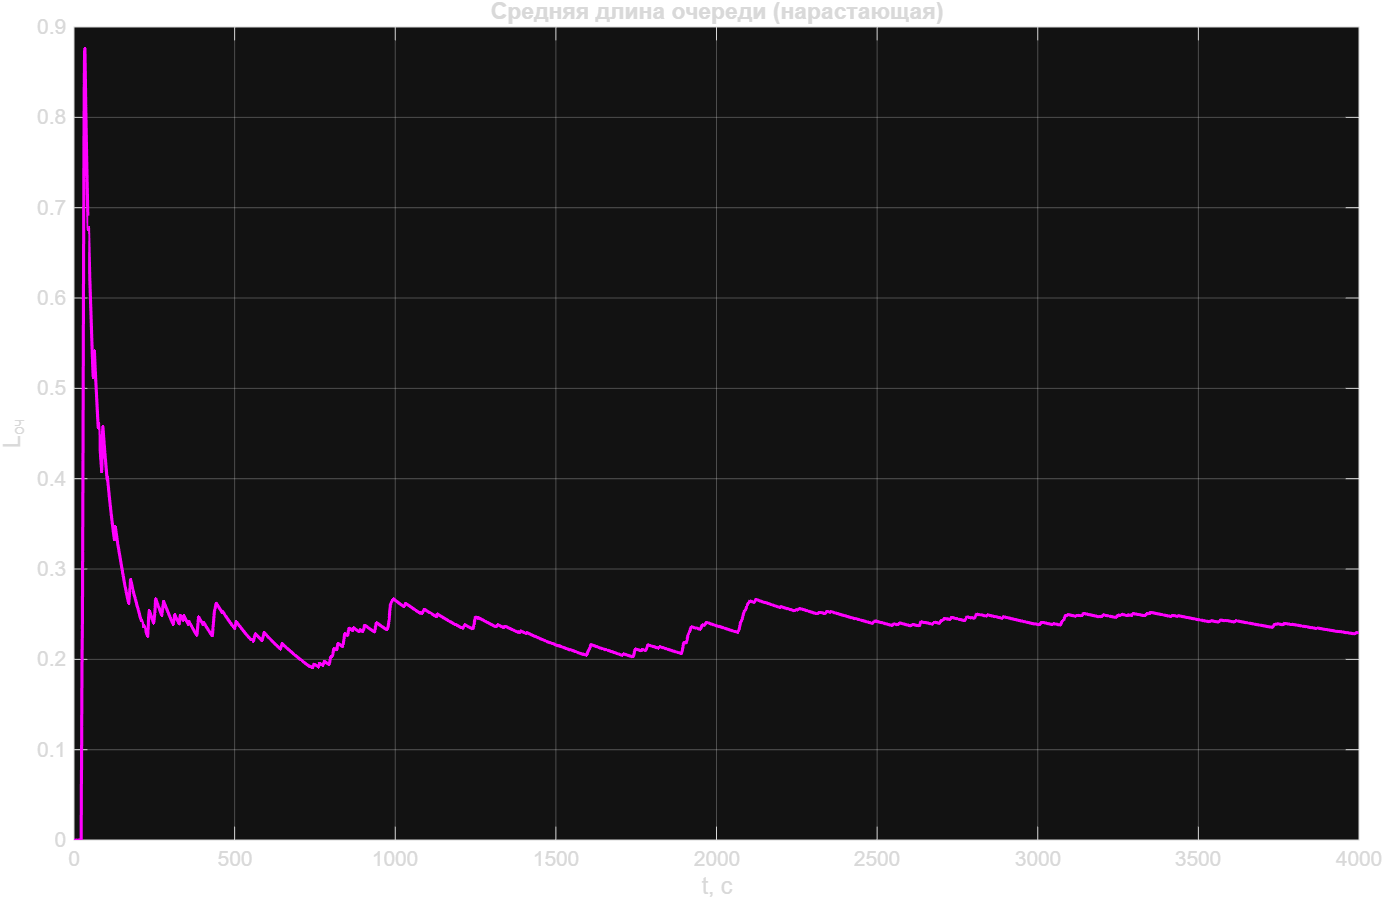
\includegraphics[width=0.9\textwidth]{lab9_fig1.png}
    \caption{Прибытия заявок в СМО (кумулятивная кривая)}
    \label{fig:lab9_arr}
\end{figure}

\begin{figure}[H]
    \centering
    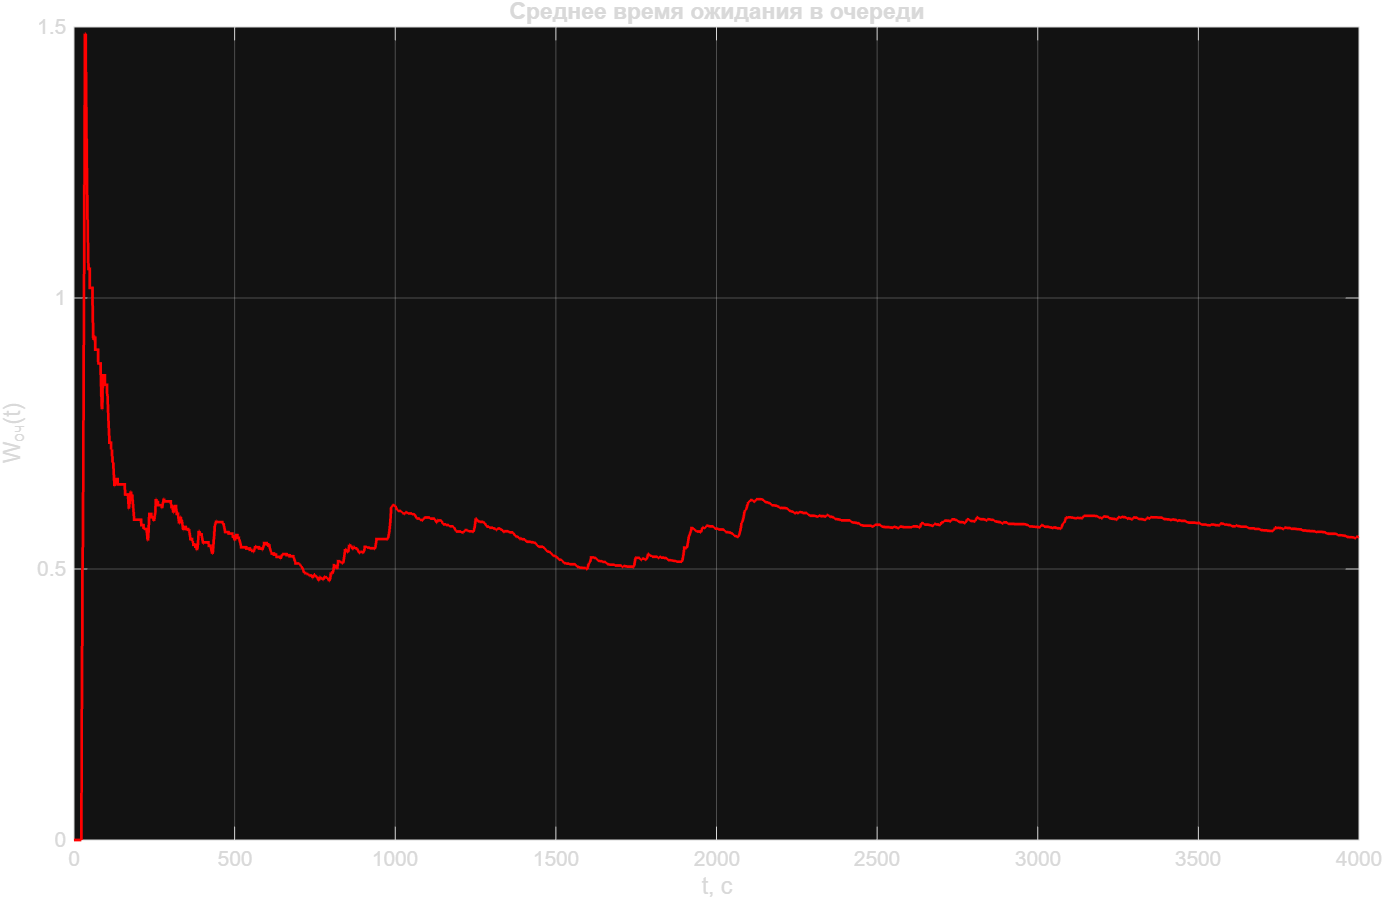
\includegraphics[width=0.9\textwidth]{lab9_fig3.png}
    \caption{Выходы (обслуженные заявки) из СМО}
    \label{fig:lab9_dep}
\end{figure}

\begin{figure}[H]
    \centering
    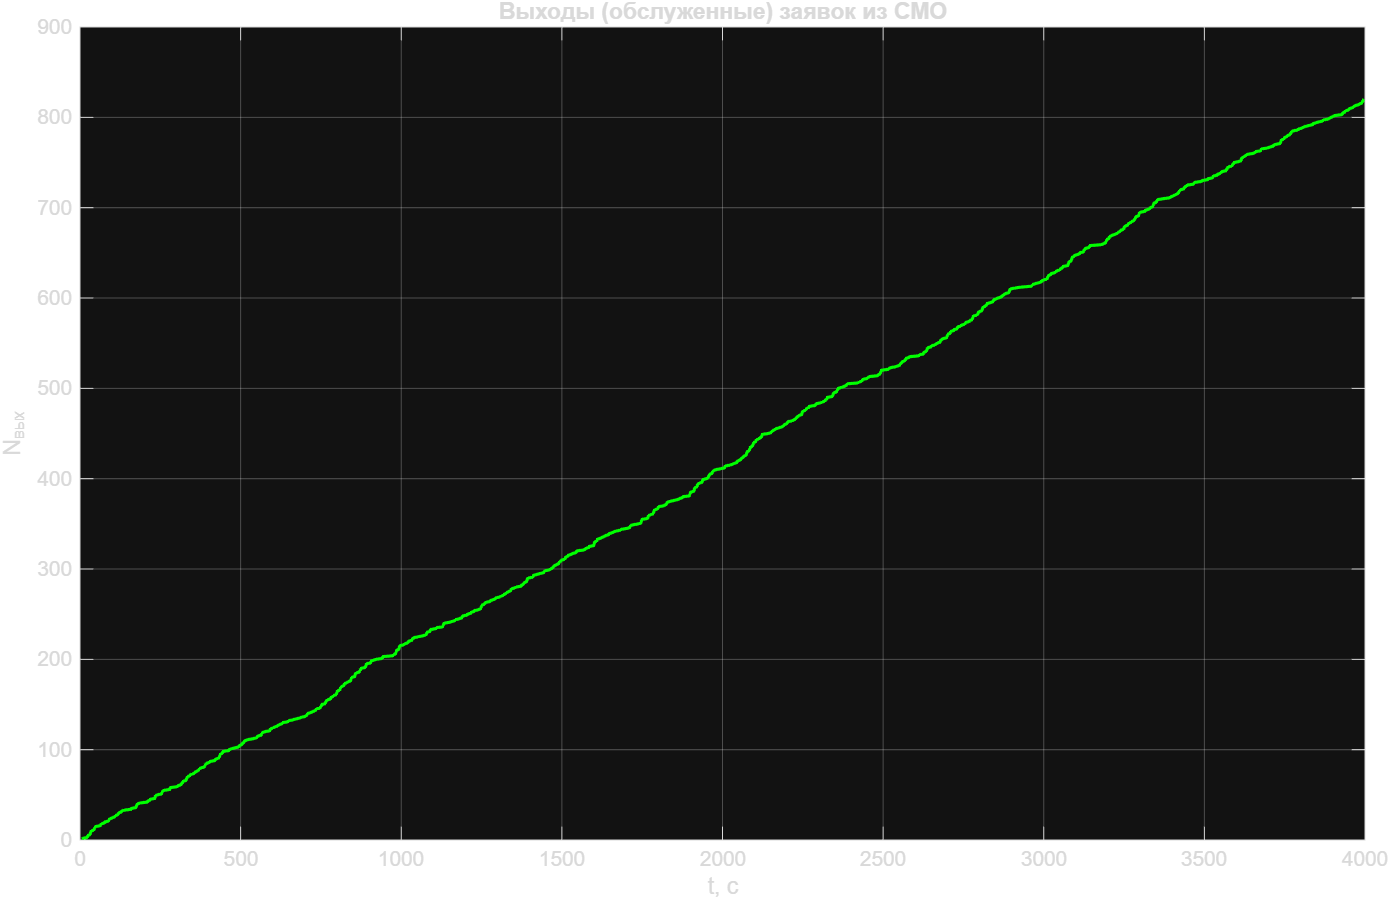
\includegraphics[width=0.9\textwidth]{lab9_fig2.png}
    \caption{Среднее время ожидания заявки в очереди (в динамике)}
    \label{fig:lab9_w}
\end{figure}

\begin{figure}[H]
    \centering
    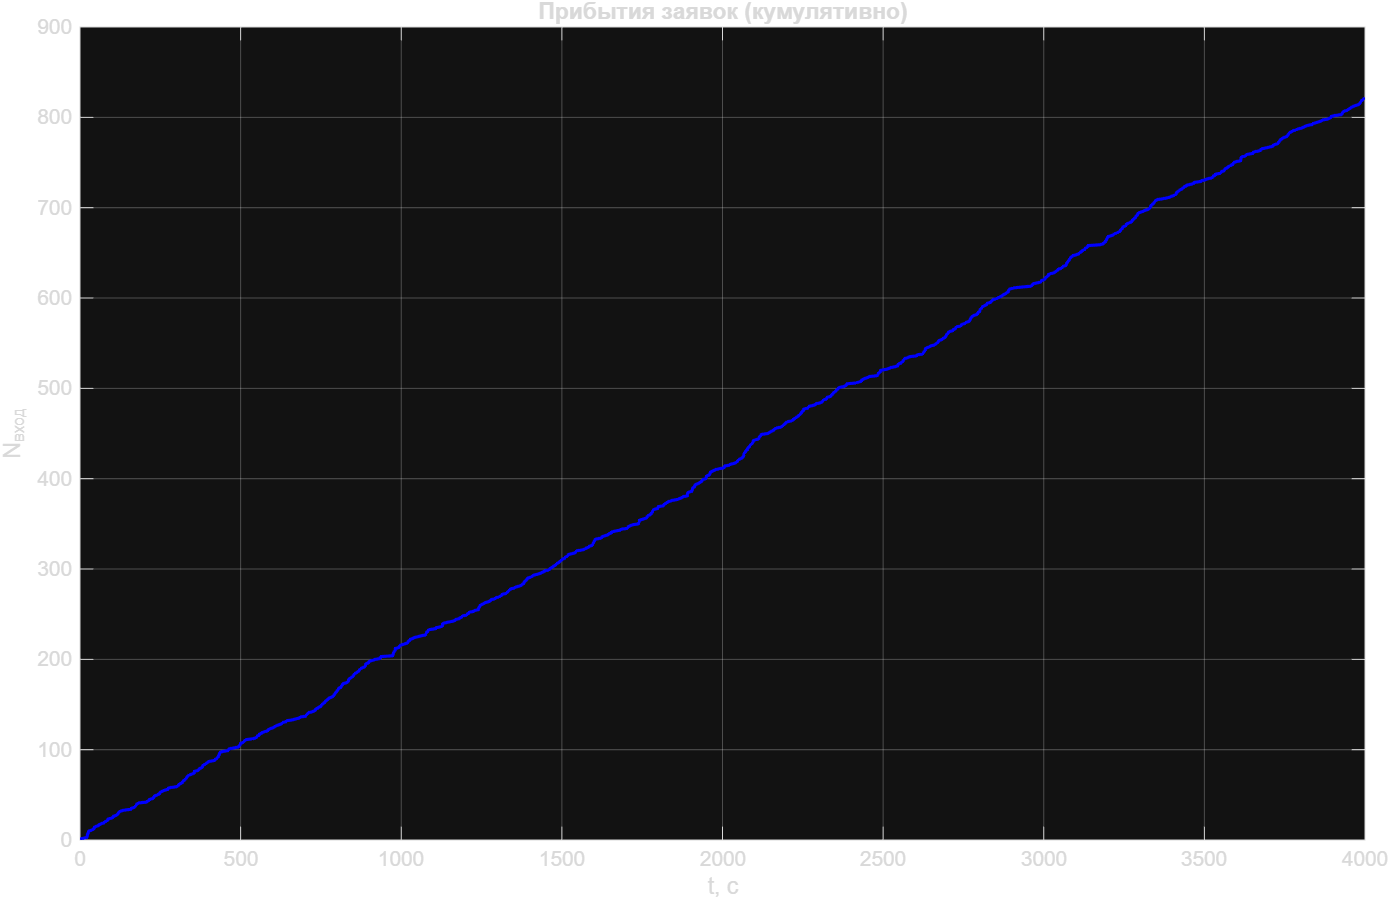
\includegraphics[width=0.9\textwidth]{lab9_fig4.png}
    \caption{Средняя длина очереди (нарастающая)}
    \label{fig:lab9_lq}
\end{figure}

\section*{Ответы на контрольные вопросы}
\begin{enumerate}
    \item \textbf{Вопрос 1. Каковы назначение и принципы функционирования пакета SimEvents в среде Simulink? } SimEvents — это расширение Simulink для моделирования систем, управляемых дискретными событиями, где модельное время перематывается скачком к моменту следующего события, а основным объектом является сущность (entity), проходящая через сеть блоков и несущая атрибуты для сбора статистики.
    \item \textbf{Вопрос 2. Каким образом в модели обеспечивается экспоненциальный закон распределения временных интервалов?} Экспоненциальное распределение строится методом обратной функции на базе равномерной случайной величины U из интервала (0, 1) по формуле Δt = -(1/λ) * ln(U), что в Simulink реализуется цепочкой блоков: генератор равномерного шума, блок натурального логарифма и усилитель с коэффициентом -1/λ.
    \item \textbf{Вопрос 3. Какова роль накопителя (Queue) и дисциплины обслуживания FIFO?} Блок Queue выполняет роль буфера, накапливающего заявки при занятости сервера и предотвращающего их потерю, а дисциплина FIFO гарантирует, что заявка, пришедшая раньше всех, будет обслужена первой, что математически означает зависимость времени ожидания только от суммарного времени обслуживания предшествующих заявок.
    \item \textbf{Вопрос 4. Каким образом организуется сбор и вычисление интегральных показателей СМО?} Интегральные показатели снимаются напрямую со статистических портов блоков SimEvents: порт Utilization сервера даёт коэффициент загрузки ρ, порты очереди выдают среднюю длину очереди и среднее время ожидания, а абсолютная пропускная способность вычисляется как отношение числа завершённых заявок к модельному времени.
\end{enumerate}

\section{Текст программы}
\begin{verbatim}
%% Лабораторная работа N9 (SimEvents).
%% ИКС-431 Салий В.П., вариант 18
mu = 1; capQ = 10; Tstop = 4000;
expParams = [0.20 1 0.5;  0.10 1 0.6;  0.30 1 0.1;
             0.10 1 0.3;  0.40 1 0.2];
for e = 1:size(expParams,1)
    res = run_smo9(expParams(e,1), expParams(e,2), ...
                   expParams(e,3), mu, capQ, Tstop);
    fprintf('A=%.4f T=%.3f Lq=%.3f rho=%.3f\n', ...
        res.A, res.T_sys, res.Lq, res.util);
end

function res = run_smo9(lambda, wmax, pfb, mu, capQ, Tstop)
    load_system('sldelib');  m = 'SMO_lab9';  new_system(m);
    n = 10;  k = round(pfb*n);
    add_block('sldelib/Entity Generator',      [m '/G']);
    add_block('sldelib/Entity Input Switch',   [m '/IS']);
    add_block('sldelib/Entity Queue',          [m '/Q']);
    add_block('sldelib/Entity Server',         [m '/S']);
    add_block('sldelib/Entity Output Switch',  [m '/SW']);
    add_block('sldelib/Entity Terminator',     [m '/T']);
    act = ['dt = -log(rand())/' num2str(lambda) ';'];
    set_param([m '/G'], 'TimeSource', 'Function', ...
        'IntergenerationTimeAction', act, ...
        'AttributeName', 'st');
    act2 = ['st = -log(rand())/' num2str(mu) ...
            ' + rand()*' num2str(wmax) ';'];
    set_param([m '/G'], 'GenerateAction', act2);
    set_param([m '/Q'], 'Capacity', num2str(capQ), ...
        'QueueType', 'FIFO');
    set_param([m '/S'], 'Capacity', '1', ...
        'ServiceTimeSource', 'Attribute', ...
        'ServiceTimeAttributeName', 'st');
    set_param([m '/SW'], 'NumberOutputPorts', num2str(n), ...
        'SwitchingCriterion', 'Round robin');
    % сущность = последний outport; статистика -> To Workspace
    add_line(m,'G/2','IS/1');  add_line(m,'IS/1','Q/1');
    add_line(m,'Q/3','S/1');   add_line(m,'S/2','SW/1');
    add_line(m,'SW/1','IS/2'); add_line(m,'SW/2','T/1');
    set_param(m,'StopTime',num2str(Tstop), ...
        'Solver','FixedStepDiscrete');
    out = sim(m);  % чтение портов статистики,
                   % расчёт A, T, Lq, rho
end
\end{verbatim}

\section*{Выводы по лабораторной работе}
\addcontentsline{toc}{section}{Выводы по лабораторной работе}
В ходе работы средствами MATLAB/Simulink и пакета SimEvents построена и протестирована модель однофазной одноканальной СМО M/M/1/10 с ограниченной очередью и обратной связью. Модель обеспечивает задание всех требуемых параметров (число заявок, интенсивность $\lambda$, максимальный вес, вероятность возврата $p$) и выдаёт полный набор характеристик: абсолютную пропускную способность, среднее время пребывания в системе, среднюю длину очереди, коэффициент загрузки и графики динамики поступлений, ожиданий и выходов.

Результаты моделирования подтверждают теоретические закономерности: рост $\lambda$ и $p$ увеличивает загрузку канала и длину очереди, а условие стационарности $\rho_\text{эф}=\lambda/[\mu(1-p)]<1$ является необходимым для устойчивой работы системы с обратной связью. Полученные значения согласуются с расчётами по формулам одноканальной СМО с ограниченной очередью и формуле Литтла.

\end{document}
